\documentclass[11pt]{article}
\usepackage[spanish, es-tabla]{babel}

\usepackage{amsmath}
\usepackage{amssymb}
\usepackage{amsthm}

\usepackage{fontspec}
\usepackage{multicol}
\usepackage{graphicx}
\usepackage{float}
\usepackage[center]{caption}
\usepackage{graphicx}
\usepackage{listings}
\usepackage[dvipsnames, table]{xcolor}
\usepackage{fancyhdr}
\usepackage{titling}
\usepackage[fixlanguage]{babelbib}
\selectbiblanguage{spanish}
\usepackage{subcaption}
\captionsetup{labelfont=bf}
% \captionsetup[table]{labelfont={bf},name={Tabla},labelsep=period}
\usepackage{hyperref}
\definecolor{blueX}{HTML}{3f84e4}
\setmonofont{SFMonoRegular.otf}
\usepackage[margin=2.8cm]{geometry}
\hypersetup{
    colorlinks,
    citecolor=black,
    filecolor=black,
    linkcolor=black,
    urlcolor=black
}
\usepackage{siunitx}
\sisetup{
    per-mode = fraction,
    detect-all,
    exponent-product = \cdot
}
\usepackage{enumitem}
\usepackage{pdflscape}
\usepackage[stylemods,style=super, nogroupskip, toc=false, hyperfirst=false, nonumberlist]{glossaries-extra}

\setlength{\parindent}{0pt} % To avoid indentation
\setabbreviationstyle[acronym]{long-short}
\makenoidxglossaries
\newglossary{difusion}{difusionin}{difusionout}{Glosario}
\loadglsentries{glosario}

% COLUMNAS Y FILAS MULTIPLES DENTRO DE TABLAS
\usepackage{multirow, hhline}
\usepackage{array}
\newcolumntype{L}[1]{>{\raggedright\let\newline\\\arraybackslash\hspace{0pt}}m{#1}}
\newcolumntype{C}[1]{>{\centering\let\newline\\\arraybackslash\hspace{0pt}}m{#1}}
\newcolumntype{R}[1]{>{\raggedleft\let\newline\\\arraybackslash\hspace{0pt}}m{#1}}
\renewcommand{\listfigurename}{Figuras}
\renewcommand{\listtablename}{Tablas}

% \renewcommand{\familydefault}{\sfdefault}
\renewcommand{\thesubsubsection}{\alph{subsubsection}}

\usepackage{titlesec}
\titleformat*{\subsection}{\normalsize\bfseries}
\titleformat*{\subsubsection}{\normalsize\bfseries}

\titlespacing\subsection{0pt}{12pt plus 4pt minus 2pt}{0pt plus 2pt minus 2pt}
\titlespacing\subsubsection{0pt}{12pt plus 4pt minus 2pt}{0pt plus 2pt minus 2pt}

\begin{document}

\title{\textbf{Informe de evaluación de ruido debido a las operaciones de vuelo del aeropuerto\\Adolfo Suárez Madrid-Barajas}}
\author{Javier Rodrigo López}
\date{\today}
\maketitle

\pagenumbering{gobble}

\fancypagestyle{firststyle}
{
    \fancyhead[L]{Acústica Ambiental}
    \fancyhead[R]{
\includegraphics[width=0.3\linewidth]{Imágenes/ETSIST.png}}
    %\fancyfoot[R]{
\includegraphics[width=0.08\linewidth]{Imágenes/Plantilla_IAC.png}\\Departamento de Ingeniería Audiovisual y Comunicaciones}
}

\thispagestyle{firststyle}

% \newpage

\fancyhead{}
\pagestyle{fancy}

\pagestyle{fancy}
\fancyhead[L]{Acústica Ambiental}
\fancyhead[R]{Curso 2024/25}

%\newpage
%\tableofcontents
%\listoffigures
\setcounter{figure}{0}
\setlength{\parskip}{0.5em}

\hypersetup{
    citecolor=black,
    filecolor=black,
    linkcolor=black,
    urlcolor=blueX
}

\tableofcontents
\listoffigures

% IMPRIME ACRÓNIMOS, SIGLAS Y GLOSARIO
%\glsaddall
%\newpage
%\printnoidxglossaries

\newpage

\pagenumbering{arabic}
\setcounter{page}{2}

\section{Introducción}

Este informe forma parte de la Práctica 1 de la asignatura de Acústica Ambiental, impartida por el departamento de Ingeniería Audiovisual y Comunicaciones de la Escuela Técnica Superior de Ingenieros de Telecomunicación de la Universidad Politécnica de Madrid.

El objetivo de este informe consiste en evaluar el ruido producido por las operaciones de vuelo del aeropuerto Adolfo Suárez Madrid-Barajas, motivado por la apertura de una nueva pista. Se han utilizado las normas \cite{ISO1996-2:2020} y \cite{ISO20906:2009} para la medición y evaluación del ruido.

\section{Ensayo}
\section{Equipos y materiales}
\section{Mediciones y resultados}

\begin{table}[htbp]
    \centering
    \caption{Indicadores de ruido de las aeronaves registradas}
    \begin{tabular}{|l|c|c|c|c|c|} \hline
        Evento                                              & Hora de inicio     & $T \, (\unit{\s})$ & $L_{Aeq,T}\, (\unit{\dB})$ & $L_{AE}\, (\unit{\dB})$ & $L_{Amax}\, (\unit{\dB})$ \\ \hline
        \rowcolor[rgb]{ .867,  .922,  .969} Aeronave 36R-1  & 20/02/2023 8:37:28 & 56                 & 69.8                       & 87.2                    & 74.3                      \\ \hline
        \rowcolor[rgb]{ .867,  .922,  .969} Aeronave 36R-2  & 20/02/2023 8:39:00 & 16                 & 77.1                       & 89.1                    & 80.3                      \\ \hline
        \rowcolor[rgb]{ .867,  .922,  .969} Aeronave 36R-3  & 20/02/2023 8:41:26 & 16                 & 78.0                       & 90.1                    & 81.6                      \\ \hline
        \rowcolor[rgb]{ .867,  .922,  .969} Aeronave 36R-4  & 20/02/2023 8:52:20 & 18                 & 77.7                       & 90.2                    & 81.6                      \\ \hline
        \rowcolor[rgb]{ .867,  .922,  .969} Aeronave 36R-5  & 20/02/2023 8:55:12 & 15                 & 80.8                       & 92.6                    & 84.5                      \\ \hline
        \rowcolor[rgb]{ .867,  .922,  .969} Aeronave 36R-6  & 20/02/2023 8:56:35 & 18                 & 77.6                       & 90.2                    & 81.7                      \\ \hline
        \rowcolor[rgb]{ .867,  .922,  .969} Aeronave 36R-7  & 20/02/2023 8:58:14 & 30                 & 74.4                       & 89.2                    & 79.2                      \\ \hline
        \rowcolor[rgb]{ .867,  .922,  .969} Aeronave 36R-8  & 20/02/2023 9:00:03 & 20                 & 79.5                       & 92.5                    & 83.8                      \\ \hline
        \rowcolor[rgb]{ .867,  .922,  .969} Aeronave 36R-9  & 20/02/2023 9:04:36 & 32                 & 73.2                       & 88.3                    & 77.9                      \\ \hline
        \rowcolor[rgb]{ .867,  .922,  .969} Aeronave 36R-10 & 20/02/2023 9:06:04 & 19                 & 79.0                       & 91.8                    & 83.1                      \\ \hline
        \rowcolor[rgb]{ .867,  .922,  .969} Aeronave 36R-11 & 20/02/2023 9:13:37 & 21                 & 73.9                       & 87.1                    & 78.4                      \\ \hline
        \rowcolor[rgb]{ .867,  .922,  .969} Aeronave 36R-12 & 20/02/2023 9:18:33 & 19                 & 74.9                       & 87.7                    & 78.9                      \\ \hline
        \rowcolor[rgb]{ .886,  .937,  .855} Aeronave 36L-1  & 20/02/2023 9:02:57 & 33                 & 72.3                       & 87.5                    & 76.1                      \\ \hline
        \rowcolor[rgb]{ .886,  .937,  .855} Aeronave 36L-2  & 20/02/2023 9:15:27 & 47                 & 69.6                       & 86.3                    & 74.6                      \\ \hline
        Ruido total                                         & -                  & -                  & 69.9                       & 104.3                   & 84.5                      \\ \hline
        Ruido 36L                                           & -                  & -                  & 70.9                       & 89.9                    & 76.1                      \\ \hline
        Ruido 36R                                           & -                  & -                  & 76.4                       & 100.8                   & 84.5                      \\ \hline
    \end{tabular}
    \label{tab:indicadores}
\end{table}

La duración de los eventos de ruido es un dato inmediato, puesto que solamente es necesario calcular la diferencia en segundos entre la hora de inicio y la hora de fin de cada evento, que han sido seleccionadas manualmente mediante la utilidad de marcadores del programa \textit{Enviro Noise Partner}. El criterio utilizado para delimitar esta zona ha sido la selección de los niveles de ruido situados en un margen de \qty{10}{\dB} con respecto al nivel máximo del evento sonoro.

Cabe mencionar que en varios de los eventos no era posible seguir este criterio, ya que el nivel residual se encontraba a menos de \qty{10}{\dB} del nivel máximo del evento sonoro. Esta situación se describe en la norma \cite{ISO20906:2009}. Uno de los eventos afectados es Aeronave 36R-1, el cual tiene una duración de \qty{56}{\s}.

\subsection{Indicadores de eventos individuales}

\subsubsection{Cálculo de $L_{Aeq,T}$}

El nivel de presión sonora equivalente ponderado $L_{Aeq,T}$ se ha calculado en base a las mediciones de $L_{AE, i}$ obtenidas con el sonómetro. A continuación se expone el cálculo para el evento Aeronave 36R-1:

\begin{equation} \label{eq:laeqt}
    L_{Aeq,T} = 10 \log \left( \frac{1}{T} \sum_{i=1}^{T} 10^{\frac{L_{AE, i}}{10}} \right) = \qty{69.8}{\dB}
\end{equation}

\subsubsection{Cálculo de $L_{AE}$}

Para obtener el nivel de exposición sonora se utiliza el valor que acabamos de conseguir:
\begin{equation} \label{eq:laeq}
    L_{AE} = L_{Aeq,T} + 10 \log \left( \frac{\Delta t}{T_0} \right) = \qty{69.8}{\dB} + 10 \log \left( \frac{56}{1} \right) = \qty{87.2}{\dB}
\end{equation}

\subsubsection{Cálculo de $L_{Amax}$}

El nivel de presión sonora máximo $L_{Amax}$ se obtiene como el valor máximo de los valores de exposición sonora correspondientes al evento sonoro.

\begin{equation}
    L_{Amax} = \max \left\lbrace L_{AE, i} \right\rbrace = \qty{74.3}{\dB}
\end{equation}

\subsection{Indicadores de eventos acumulados}

Los indicadores acumulados que se han calculado son el nivel de ruido total, el nivel de ruido en la pista 36L y el nivel de ruido en la pista 36R. También se podría haber calculado el nivel de ruido residual, que consistiría en excluir los eventos de ruido específicos de la medida total.

\subsubsection{Cálculo de $L_{Aeq,T}$}

Este indicador se ha calculado usando la \autoref{eq:laeqt}, pero incluyendo todos los eventos de ruido, incluyendo los eventos de ruido de la pista 36L, e incluyendo los eventos de ruido de la pista 36R, respectivamente.


\subsection{Espectro del evento Aeronave 36L-1}
\begin{table}[htbp]
    \centering
    \caption{Espectro del evento Aeronave 36L-1}
    \begin{tabular}{|l||c|c|c|c|c|c|c|c|}
        \hline
        Banda                       & \qty{12.5}{\hertz}      & \qty{16}{\hertz}     & \qty{20}{\hertz}     & \qty{25}{\hertz}       & \qty{31.5}{\hertz}      & \qty{40}{\hertz}       & \qty{50}{\hertz}        & \qty{63}{\hertz}       \\ \hline
        $L_{Zeq,T} \, (\unit{\dB})$ & 61.7                    & 67.6                 & 65.9                 & 65.1                   & 66.2                    & 66.6                   & 67.2                    & 68.0                   \\ \hline \hline
        Banda                       & \qty{80}{\hertz}        & \qty{100}{\hertz}    & \qty{125}{\hertz}    & \qty{160}{\hertz}      & \qty{200}{\hertz}       & \qty{250}{\hertz}      & \qty{315}{\hertz}       & \qty{400}{\hertz}      \\ \hline
        $L_{Zeq,T} \, (\unit{\dB})$ & 65.9                    & 63.6                 & 66.7                 & 68.2                   & 67.3                    & 62.7                   & 66.4                    & 66.9                   \\ \hline \hline
        Banda                       & \qty{500}{\hertz}       & \qty{630}{\hertz}    & \qty{800}{\hertz}    & \qty{1}{\kilo\hertz}   & \qty{1.25}{\kilo\hertz} & \qty{1.6}{\kilo\hertz} & \qty{2}{\kilo\hertz}    & \qty{2.5}{\kilo\hertz} \\ \hline
        $L_{Zeq,T} \, (\unit{\dB})$ & 66.3                    & 63.2                 & 64.3                 & 64.3                   & 62.9                    & 61.0                   & 58.1                    & 53.0                   \\ \hline \hline
        Banda                       & \qty{3.15}{\kilo\hertz} & \qty{4}{\kilo\hertz} & \qty{5}{\kilo\hertz} & \qty{6.3}{\kilo\hertz} & \qty{8}{\kilo\hertz}    & \qty{10}{\kilo\hertz}  & \qty{12.5}{\kilo\hertz} & \qty{16}{\kilo\hertz}  \\ \hline
        $L_{Zeq,T} \, (\unit{\dB})$ & 46.6                    & 40.5                 & 33.3                 & 27.8                   & 20.8                    & 12.4                   & 5.5                     & 2.9                    \\ \hline \hline
        Banda                       & \qty{20}{\kilo\hertz}   &                      &                      &                        &                         &                        &                         &                        \\ \hline
        $L_{Zeq,T} \, (\unit{\dB})$ & 3.8                     &                      &                      &                        &                         &                        &                         &                        \\ \hline
    \end{tabular}
    \label{tab:espectro_36L-1}
\end{table}


\begin{figure}[htp]
    \centering
    \caption{Espectro del evento Aeronave 36L-1}
    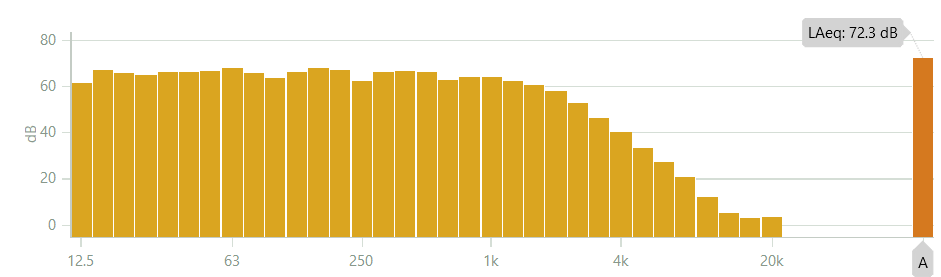
\includegraphics[width=\linewidth]{Imágenes/espectro.png}
    \label{fig:Espectro_36L-1.png}
\end{figure}

\subsection{Percentiles}

\section{Conformidad con la legislación vigente}


\nocite{*}
\newpage
\bibliography{Bibliography}
\bibliographystyle{IEEEtr}

\end{document}
